\documentclass[%
	%draft,
	%submission,
	%compressed,
	final,
	%
	%technote,
	%internal,
	%submitted,
	%inpress,
	%reprint,
	%
	%titlepage,
	notitlepage,
	%anonymous,
	narroweqnarray,
	inline,
	twoside,
	%invited,
	]{ieee}

\title{Redes TP1}

\newcommand{\latexiie}{\LaTeX2{\Large$_\varepsilon$}}
\renewcommand{\abstractname}{Sinopsis}

%\usepackage{ieeetsp}	% if you want the "trans. sig. pro." style
%\usepackage{ieeetc}	% if you want the "trans. comp." style
%\usepackage{ieeeimtc}	% if you want the IMTC conference style

% Use the `endfloat' package to move figures and tables to the end
% of the paper. Useful for `submission' mode.
%\usepackage {endfloat}
% Use the `endfloat' package to move figures and tables to the end
% of the paper. Useful for `submission' mode.
%\usepackage {endfloat}

% Use the `times' package to use Helvetica and Times-Roman fonts
% instead of the standard Computer Modern fonts. Useful for the 
% IEEE Computer Society transactions.
%\usepackage{times}
% (Note: If you have the commercial package `mathtime,' (from 
% y&y (http://www.yandy.com), it is much better, but the `times' 
% package works too). So, if you have it...
%\usepackage {mathtime}

% for any plug-in code... insert it here. For example, the CDC style...
%\usepackage{ieeecdc}

%http://en.wikibooks.org/wiki/LaTeX/Importing_Graphics
\usepackage{pdfpages}
\usepackage{graphicx}

%http://en.wikibooks.org/wiki/LaTeX/Floats,_Figures_and_Captions#Wide_figures_in_two_column_documents
\usepackage{dblfloatfix}
\usepackage{fixltx2e}

%http://en.wikibooks.org/wiki/LaTeX/Floats,_Figures_and_Captions#Keeping_floats_in_their_place
\usepackage{float}
\usepackage{placeins}

%http://tex.stackexchange.com/questions/25414/how-to-create-magnified-subfigures-and-corresponding-boxes-for-portions-of-a-lar
\input{zoomboxarray}

%Bibliografia
\usepackage[backend=biber,style=numeric-comp]{biblatex}
\bibliography{ieeecls.bib}

\begin{document}

\includepdf{Caratula_Redes_TP1.pdf}
%\begin{figure*}
%	\centering
%	\includegraphics[width=\linewidth]{Caratula_Redes_TP1.pdf}
%\end{figure*}
%\FloatBarrier

%\firstpage{1}

%\confplacedate{Ciudad Aut\'onoma de Buenos Aires, Argentina, 29 de Septiembre de 2014}

\begin{abstract}
	Concentrados en el alcance de la materia, se nos presenta un trabajo
a realizar para poder familiarizarnos con los primeros an\'alisis
de la informaci\'on que nos proporciona una \textit{red} inform\'atica.

\par Nos refer\'imos por \textit{red} a la interconexi\'on de distintas
	computadoras (o tambi\'en llamadas terminales de la red) y su 
    comunicaci\'on mediante estas conexiones. Nuestro estudio se 
    concentra en un protocolo utilizado por las terminales para poder
    identificar a otras terminales con el objetivo de poder comunicarse
    entre si.
    
\par Este protocolo llamado \textit{ARP} funciona mediante el env\'io de
	un \textit{paquete}\footnote{Llamamos paquete a una cierta informaci\'on
    que respeta ciertos protocolos que todas las terminales de la red
    comprenden y respetan.} a todas las otras terminales de la red.

\par El objetivo de este trabajo es poder observar dichos paquetes (o
	dicho de otra manera, escuchar dichas comunicaciones entre participantes
    de esta red) y hacer un an\'alisis de los mismos, esperando encontrar
    informaci\'on sobre el comportamiento, topolog\'ia u cualquier otra
    caracter\'istica que nos pueda resultar \'util, siempre dentro del
    alcance del trabajo acad\'edmico que se nos pide.
\end{abstract}

%\begin{keywords}
%Style file, \latexiie, Microsoft Word, IEEE Publications, Instrumentation
%and Measurement Technology Conference, IMTC.
%\end{keywords}

\section*{Introducci\'on y Aclaraciones}\label{sec:introduccion}
	\IEEEPARstart{A}{} la hora de trabajar y analizar el comportamiento del protocolo
respecto de la congesti\'on, es inmediato dirigirnos hacia el mecanismo (si lo
hay) implementado por el protocolo con este prop\'osito.

\par El primer dato importante a mencionar, es que el protocolo PTC s\'olo replica
la estimaci\'on del RTO del mecanismo de control de congesti\'on de TCP\cite{rfc5681}.
Este valor se utiliza para determinar cuanto tiempo esperar antes de considerar que un
paquete se perdi\'o y iniciar el proceso de retransmici\'on (b\'asicamente se
utiliza para determinar un \textit{timeout}).

\par El par\'ametro por defecto que uno puede pensar para calcular el RTO, y
que efectivamente se utiliza, es el \textit{RTT}\cite{rfc1323}\cite{karns_algorithm}\cite{rfc6298},
a partir del cual se calcula el \textit{SRTT} (\textit{Smoothed Round
Trip Time}\cite{rfc6298}). As\'i pues a la hora de estimar el RTO, se
utilizan el RTT y el SRTT, en conjunto con 2 constantes denominadas \emph{alpha}
y \emph{beta}\footnote{De ahora en m\'as $\alpha$ y $\beta$.}\cite{rfc6298}.

\par Entonces, explicado esto, ya se ve de donde salen\footnote{Y de donde el
TP sugiere.} las primeras variables que iremos analizando a la hora de ver como
se comporta el protocolo: $\alpha$ y $\beta$.

\par Nos queda ahora el problema de encontrar un entorno lo suficientemente estable
que nos permita analizar el comportamiento de manera justa. El problema aqu\'i
es que debemos comenzar a simular la congesti\'on de la red, con lo cual se
nos plantea el objetivo de introducir en el protocolo un delay
$\delta$ y una probabilidad $\phi$ de p\'erdida/$dropeo$ de los paquetes. 
Se puede pensar que a mayor $\delta$ y $\phi$ se estar\'a replicando un
escenario con mayor congesti\'on. Obviamente, esto tiene sentido
en un entorno que mantenga las dem\'as variables de la red lo suficientemente
estables para que podamos asumir que la simulaci\'on de la congesti\'on es
correcta.

%-------------------------------------------------------------------------------


\section*{Sobre la herramienta de \textit{sniffing}}
	\PARstartCal El desarrollo de la herramienta que se encarga de capturar
	los paquetes ARP de la red (o m\'as comunmente dicho: \textit{sniffear})
    no, claramente, el objetivo central de este trabajo. De hecho, las
    herramientas para realizar dicha tarea quedaron a elecci\'on de todos
    los grupos de la cursada.
    
\par Nosotros, por comodidad o experiencia en el lenguaje \textit{C/C++},
	decidimos utilizar \'este para realizar esta tarea.
    
\par Se entrega con este informe (en su versi\'on digital) el c\'odigo
	fuente utilizado con su correspondiente Makefile para poder compilarlo,
    llegada la necesidad de probar el mismo.
    
\par Como librer\'ias externas al c\'odigo, se utiliz\'o la \textit{libpcap},
	quiz\'as la librer\'ia m\'as utilizada por diversos softwares open source
    que se encuentran hoy d\'ia para interactuar con los dispositivos de red
    de las computadoras y observar el tr\'afico de paquetes que atraviesan/procesan
    los mismos.
    
\par Durante el desarrollo de esta herramienta, observamos que se iba a necesitar
	el \textit{timestamp} de cada dato observado para luego poder realizar un
    an\'alisis de las diferentes redes \textit{sniffeadas} en cuanto a la variable
    temporal. Por lo tanto, dicho dato fue tambi\'en guardado en la salida de
    nuestra aplicaci\'on.
    
\par Tambi\'en se program\'o una m\'ini-aplicaci\'on en el mismo lenguaje con
	el objetivo de poder procesar los datos capturados por la aplicaci\'on ya
    descripta y calcular (en otro archivo) las probabilidades de cada s\'imbolo
    de nuestras fuentes de informaci\'on (en este caso, las direcciones IP ser\'ian
    los s\'imbolos de nuestras dos fuentes) y con estos datos tambi\'en calcular
    la entrop\'ia de ambas fuentes.

\section{Escenario 1}
	\IEEEPARstart{E}{N} este primer escenario seleccionamos una universidad ubicada
en este mismo continente (Am\'erica), con la particularidad de que la misma
se encuentra a una distancia m\'as que considerable\footnote{9024.25 km} de
Buenos Aires. La universidad en cuesti\'on es McGill\cite{mcgill} y se encuentra
en \emph{Montr\'eal, Canada}

\par El experimento en este escenario se bas\'o en utilizar la herramienta
desarrollada para realizar 1000 pedidos de \emph{rastrearutas} al host de la
p\'agina web de la universidad seleccionada. Dicho experimento se realiz\'o
durante un d\'ia iniciando a las 00, 04, 09, 12, 16 y 20 hs (hora local Argentina,
\textit{GMT-3}).

\subsection{Resultados para el total de los Experimentos}
\par Luego de realizar los experimentos descriptos, se obtuvieron en total
6000 \textit{corridas} de la aplicaci\'on desarrollada. Como ya se explic\'o
en la \textit{\nameref{sec:introduccion}}, durante todas estas corridas se
obtivieron distintas secuencias/caminos de H\textit{hops}. As\'i pues,
el primer an\'alisis realizado fue determinar cu\'antas veces se hab\'ian
obtenido las mismas secuencias:

\begin{table}[h]
    \centering
    \begin{tabular}{r | r | r}
            &\#caminos  & \\
        ids &Distintos  &\#Veces\\
        \hline\hline
        1& 36& 1\\
        37& 19& 2\\
        56& 5& 3\\
        61& 5& 4\\
        66& 1& 6\\
        67& 1& 9\\
        68& 2& 10\\
        70& 2& 11\\
        72& 2& 12\\
        74& 2& 13\\
        76& 2& 14\\
        78& 1& 15\\
        79& 1& 17\\
        80& 1& 22\\
        81& 1& 30\\
        82& 1& 35\\
        83& 1& 61\\
        84& 1& 76\\
        85& 1& 80\\
        86& 1& 98\\
        87& 1& 128\\
        88& 1& 138\\
        89& 1& 159\\
        90& 1& 294\\
        91& 1& 1563\\
        92& 1& 3040\\
        \hline\hline
    \end{tabular}
    \bigskip
    \caption{Frecuencia por \emph{path} de hops obtenida}
    \label{tab:mcgill_sec_hops}
\end{table}

\par Podemos observar que como resultado de nuesta experimentaci\'on (6000
expermientos corridos durante todo un d\'ia), a pesar de saber de que IP
no nos asegura un camino de hops para llegar al destino, es notable la diferencia
entre 2 o 3 secuencias que son el resultado de de cas\'i todo el experimento:
entre las rutas muestrales 90, 91 y 92 se tienen 4897 experimentaciones (%
aproximadamente un 80\% del total de la experimentaci\'on). Es decir, a pesar
de lo variable que puede ser la red a la hora de encontrar un camino entre 2
hosts sobre el protocolo IP (y con todas las posibles combinaciones de hops que
se podr\'ian obtener al tener en cuenta lo explicado en \emph{\nameref{sec:datos_analizados},
\nameref{sec:introduccion}}), se observa cierta predictibilidad en este proceso,
d\'andonos a entender que es muy pobable que esta sea la ruta real m\'as com\'un
que har\'an los paquetes al establecerse una comunicaci\'on entre los hosts
de origen y destino.

\par De hecho, podemos observar estos datos como una fuente de informaci\'on
donde se puede pensar que las distintas secuencias de hops como los s\'imbolos
de la fuente. De esta manera podemos determinar la entrop\'ia de la posible
ruta que se recibir\'a de realizar el \textit{rastrearutas}.

\begin{table}[h]
    \centering
    \begin{tabular}{c | c}
                   & Concentrac\'ion\\
                   & de Probabilidad\\
       Entrop\'ia   & de Rutas 90, 91 y 92\\
       \hline\hline
       2.49631 & $81,6166\%$\\
       %\hline\hline
   \end{tabular}
   \bigskip
   \caption{Entrop\'ia de la fuente de Rutas}
   \label{tab:mcgill_entropia}
\end{table}

\par Efecttivamente, como se esperaba, nos encontramos con un valor de entrop\'ia
bastante bajo\footnote{Al menos, comparado con los resultados obtenidos en el
\textit{TP1}.}

\par Continuando, en este trabajo nos centramos en el estudio de los
\textit{Round Trip Time} de los distintos hops. Como ya se explic\'o en la 
introducci\'on, no haremos foco en aquellas secuencias de hops que aparecen
con menor frecuencia. As\'i pues, exponemos los RTTs obtenidos
entre la m\'aquina de origen donde fue corrido el experimento y los hops que
respondieron para la secuencia m\'as obtenida\footnote{La secuencia 92 que 
obtuvimos en 3040 experimentos, p\'agina \pageref{tab:mcgill_sec_hops}.}.

\par En la figura \ref{fig:rtt_dev_mcgill} se observan el valor medio del RTT y
su varianza por cada hop, m\'as los resultados de las diferentes mediciones:

\begin{figure}
    \centering
    \includegraphics[width=0.5\textwidth
                    ]{img/escenario1/{mcgill_3040.path.92.rtt_acum}.pdf}
    \caption{RTT media/Desv\'io Standad}
    \label{fig:rtt_dev_mcgill}
\end{figure}

\par Como toda experimentaci\'on con casos reales (internet en este caso) nos
encontramos con resultados que distan de lo esperado teor\'icamente. Idealmente
se hubiera esperado encontrar una secuencia creciente de RTTs para los hops,
pero por los motivos ya expuestos en la \textit{\nameref{sec:introduccion}},
nos encontramos con un entorno donde el primer resultado que salta a la vista
es una serie consecutiva y considerable\footnote{La mitad de los hops.} de hops
que tienen un RTT 
\begin{enumerate*}[label=\itshape\alph*\upshape)]
    \item muy similar, con oscilaciones peque\~nas entre pares de hops
        consecutivos (del hop 10 al hop 16), y m\'as curioso a\'un

    \item para todos estos nodos (m\'as algunos m\'as) se obtuvo un RTT
        menor al RTT del \'ultimo hop (es decir, nuestro host destino).
\end{enumerate*}

\par En el caso \emph{a}, y extendiendo
lo siguiente a los \'ultimos 4 hops ya que estos tienen RTTs similares, es
de suma utilidad observar las posibles ubicaciones geogr\'aficas de los hops,
para observar si estos se encuentran en la misma ciudad (en cuyo caso los
resultados obtenidos ser\'ian razonables, ya que la distancia f\'isica entre
dos nodos de la red es directamente proporcional al RTT, c\'omo se explic\'o
en las clases te\'oricas\footnote{A pesar de que en una red
IP bien se podr\'ian tener dos hosts en la misma ciudad con RTTs extremadamente
distintos, aunque normalmente esto se deber\'ia a las configuraciones de los hops/%
\textit{gateways} intermedios.}).

\begin{figure}
    \centering
    \includegraphics[trim= 2.5cm 6.5cm 10cm 5cm,
                    clip,
                    width=0.4\textwidth
                    ]{img/escenario1/{mcgill_3040.path.92.map}.pdf}
    \caption{Distribuci\'on Geogr\'afica de los Hops}
    \label{fig:map_mcgill}
\end{figure}

\par Podemos observar entonces en la figura \ref{fig:map_mcgill} como existe
un gran hop que cubre mucha distancia (entre los EEUU y la Argentina), mientras
que luego, todos los hops se dan entre hosts ubicados mucho m\'as cerca entre
ellos (entre la costa este de EEUU, principalmente al norte, y la regi\'on
sur este de Canada).

\par Dada esta ubicaci\'on de los hops encontrados, es razonable obtener los
resultados en cuesti\'on. En primer lugar ya que es l\'ogico (y hasta deseable%
\cite{cdn}) que hops que se encuentran todos a gran distancia del host a partir
del cual se miden el RTT den resultados similares, ya que la diferencia de
1000km\footnote{Distancia aproximada entre el centro y northe de EEUU} entre hops
no es tan significante si se tiene en cuenta un salto previo de 8000km para llegar
desde la Argentina a ambos hosts\footnote{M\'as a\'un teniendo en cuenta el
\textit{overhead} en los tiempos medidos agregado por \textit{Scapy}
y los posibles esquemas de prioridades que pueden implementar los \textit{gateways/hops}
tanto para el protocolo ICMP como para el origen o destino -Argentina/Canada- de
los paquetes, como se explic\'o en la secci\'on \textit{\nameref{sec:introduccion}}.}.

\par A la hora del an\'alisis para detectar enlaces relevantes, toda esta secuencia
de hops cercanos geogr\'aficamente (al menos as\'i todo pareciera indicarlo)
no nos es particularmente relevante (justamente, por el an\'alisis reci\'en hecho
sobre ellos vemos que no son relevantes en cuanto al $RTT_i$ entre ellos). A
su vez, estas oscilaciones nos perjudicaran al utilizar el $ZScore$ para comparar
los $RTT_i's$ de todos los dem\'as nodo (tal como ya se explic\'o al comienzo de
este trabajo). As\'i pues, al filtrar aquellos hops que no nos suman mucho
con nuestro objetivo (ya que las oscilaciones nos dar\'an $RTT_i's$ negativos),
se obtiene la figura \ref{fig:rtt_dev_mcgill_filtered}, que no es otra cosa que
los $RTTs$ de los hops que ser\'an analizados con el $ZScore$.

\begin{figure}
    \centering
    \includegraphics[width=0.5\textwidth
                    ]{img/escenario1/{mcgill_3040.path.92.rtt_acum_filtered}.pdf}
    \caption{RTT media/Desv\'io Standad para $Hops$ Relevantes}
    \label{fig:rtt_dev_mcgill_filtered}
\end{figure}

\par Tambi\'en se puede observar en este subconjunto de hops que evaluaremos
en lo que resta de este escenario que el hop 8 fue filtrado. Se puede observar
que el mismo es el hop con mayor desv\'io est\'andard (ergo, mayor variabilidad
de sus tiempos de respuesta). A su vez, el $RTT$ promedio que nos di\'o es
mayor al de su hop consecutivo, que tiene un desv\'io mucho menor. Por lo tanto,
conclu\'imos que este hop se comportaba m\'as como un $outlier$ en cuanto
al an\'alisis de enlaces relevantes, que es el foco de este trabajo.

\par Ya habiendo filtrado aquellos hops que no nos presentan informaci\'on
relevante para detectar los enlaces submarinos, se presenta en la figura
\ref{fig:zscore_mcgill_filtered} el resultado de los $ZScore$ para cada
uno de estos hops:

\begin{figure}
    \centering
    \includegraphics[width=0.5\textwidth
                    ]{img/escenario1/{mcgill_3040.path.92.rtti_zscore_filtered}.pdf}
    \caption{$ZScore$ por $RTT_i$}
    \label{fig:zscore_mcgill_filtered}
\end{figure}


\section{Escenario 2}
	\subsection{Descripci\'on del Escenario}
	\par Al igual que el escenario anterior, esta es una red laboral, pero con características muy diferentes. La red pertenece a una oficina de desarrollo de software y hardware con 14 personas. También hay un servidor de archivos, uno con maquinas virtuales y uno con bases de datos, 1 bridge wireless (independiente del router) y varios dispositivos de hardware conectados a la misma. La red es 10.10.0.0/24, teniendo el gateway la IP 10.10.0.1. 
	 \par Se capturaron paquetes arp durante 5 horas, mediante una interfaz de red Ethernet.
     
\subsection{An\'alisis de datos obtenidos}
	\par Comenzamos realizando un grafo dirigido, en el cual los nodos son las direcciones IP, y los ejes representan pedidos arp ("who-has") de una IP fuente a una IP destino.
	\begin{figure}[H]
		\centering
		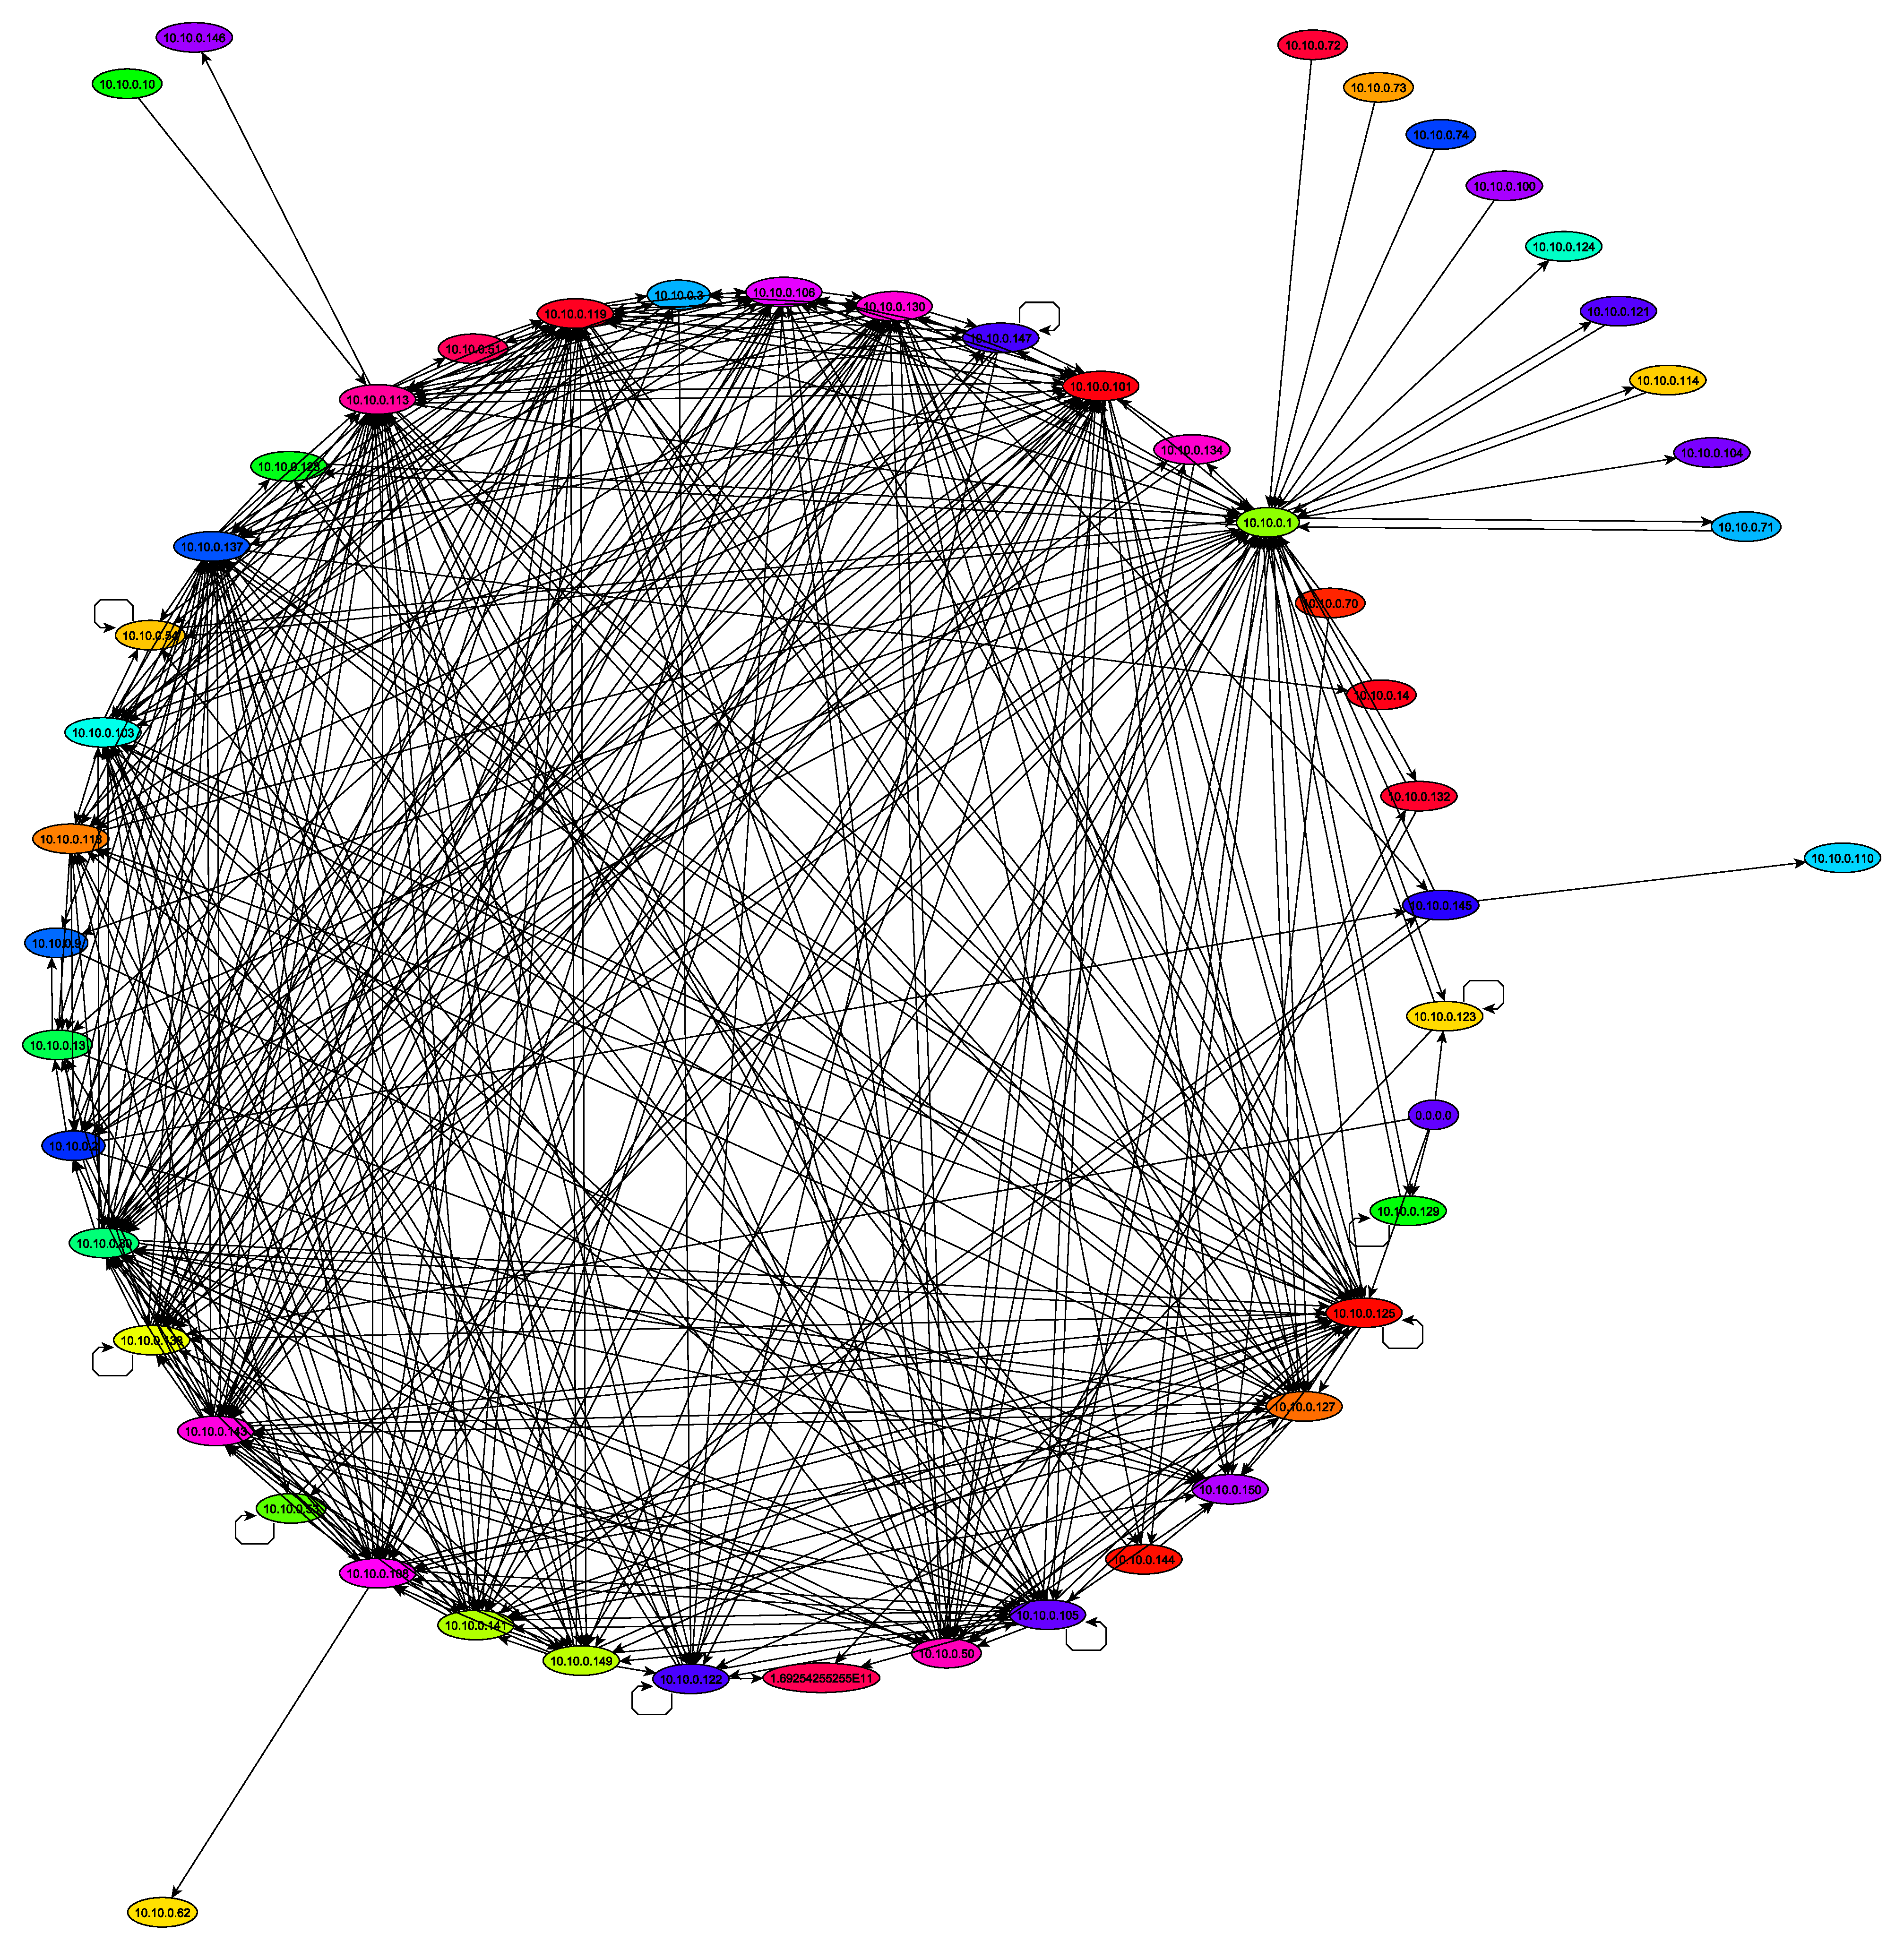
\includegraphics[width=0.5\textwidth]{img/graph/escenario_2/grafico_de_la_red.eps}
		\caption{Grafo de la red del Escenario 2}
		\label{fig:grafo_escenario2}
	\end{figure}
    
    A simple vista, este grafo no nos aporta demasiada información, pero el hecho de que sea una única gran componente conexa se corresponde con la configuración de la red. Inspeccionando las etiquetas de los nodos, observamos que efectivamente, todas las direcciones se encuentran en el rango 10.10.0.1-10.10.0.254, con excepción de dos casos particulares: la IP 0.0.0.0 y la IP 169.254.255.255. Más adelante nos concentraremos en estas dos direcciones. 
    \par Lo primero que nos interesó ver fue cuales fueron las IPs más pedidas, y cuales fueron las que más pedidos realizaron. Para esto, realizamos histogramas que reflejan visualmente esto:
    \begin{figure}[H]
		\centering
		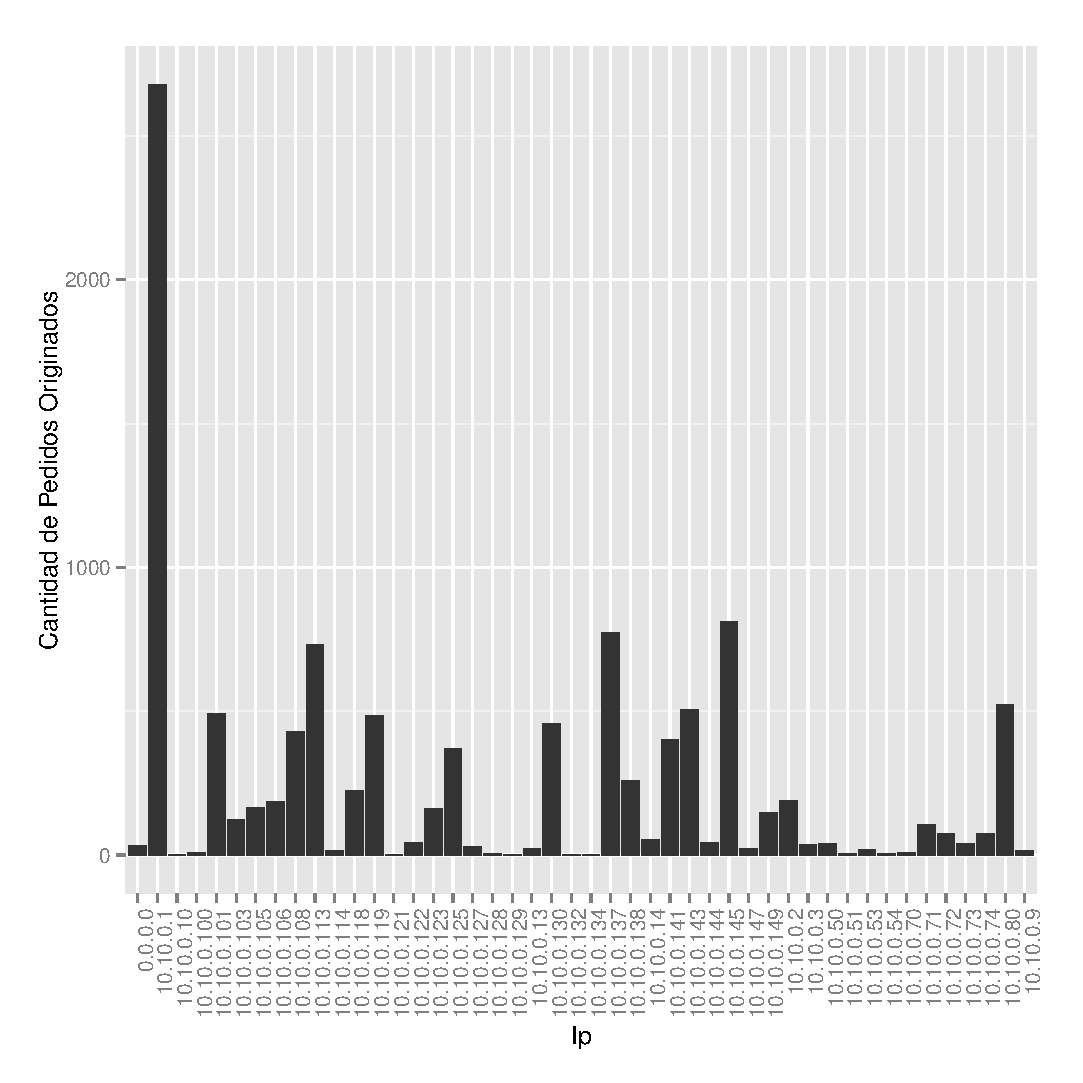
\includegraphics[width=0.5\textwidth]{img/graph/escenario_2/histogramSrc.eps}
		\caption{Escenario 2 - Histograma Origen}
		\label{fig:escenario2_histogramaSrc}
	\end{figure}       
    En este histograma podemos observar que hay una IP que predomina ampliamente sobre las demás, la 10.10.0.1, casualmente la del gateway. El resto se encuentra bastante distribuido. Hay 25 IPs que realizaron menos de 100 pedidos, 15 que realizaron entre 100 y 500, 5 que realizaron entre 500 y 1000 y el caso excepcional de la 10.10.0.1 que realizo 2678. Rapidamente nos dimos cuenta de no ibamos a obtener demasiada información sobre la red mirando quien origina los pedidos, porque lo importante es cuales son más solicitadas.
       
    \begin{figure}[H]
		\centering
		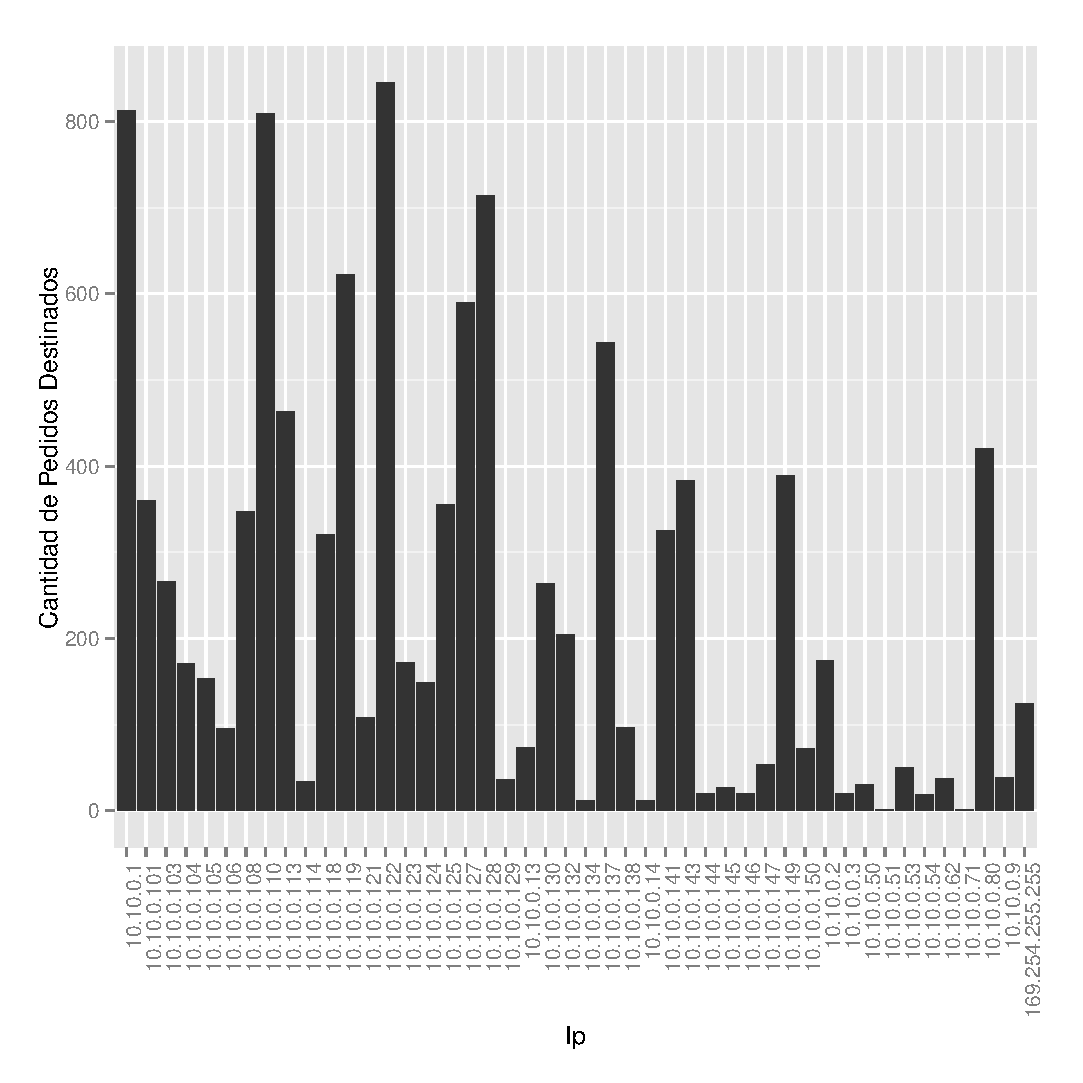
\includegraphics[width=0.5\textwidth]{img/graph/escenario_2/histogramDst.eps}
		\caption{Escenario 2 - Histograma Destino}
		\label{fig:escenario2_histogramaDst}
	\end{figure}
            
    \par En este otro histograma se ve una mayor distribución de los pedidos. Hay algunas IP que casí no cuentan con pedidos, mientras que hay muchas que cuentan con más de 100. Concretamente hay 20 IPs que fueron pedidas menos de 100 veces, 19 entre 100 y 500 veces y 7 pedidas entre 500 y 845 veces.
    Decidimos tomar las 5 IPs que fueron pedidas mayor cantidad de veces, para ver si nos aportaban alguna información valiosa:
        
    \begin{table}[H]
		\caption{Escenario 2 - IPs más pedidas}
		\centering
		\begin{tabular}{c c}
          IP & Cantidad de pedidos \\
          \hline 
          10.10.0.122 & 845 \\ 
          10.10.0.1 & 813 \\
          10.10.0.110 & 809 \\
          10.10.0.128 & 714 \\
          10.10.0.119 & 622 \\   
  		\end{tabular}
  	\end{table}
    
    En base a esto, buscamos en el grafo las vecindades de los nodos correspondientes a estas IPs:
    \begin{figure}[H]
		\centering
		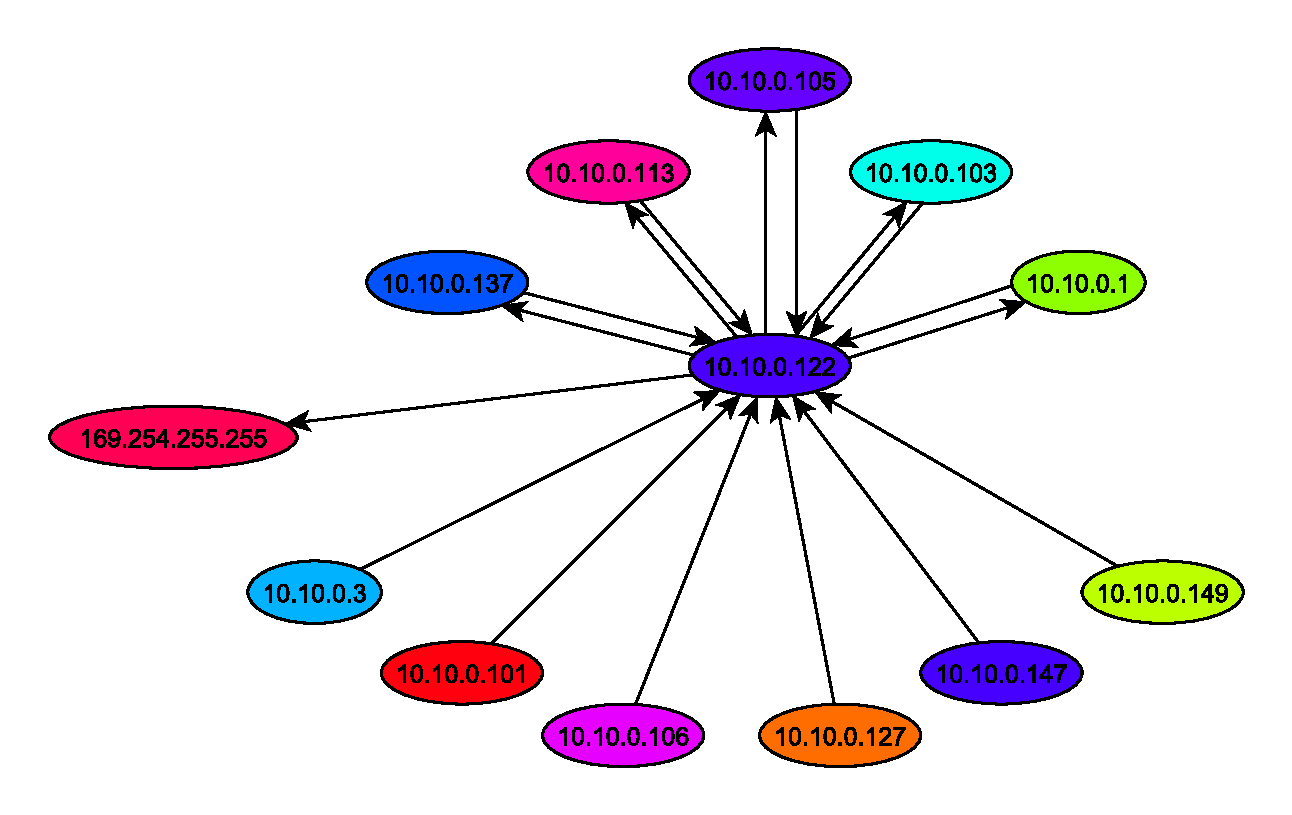
\includegraphics[width=0.5\textwidth]{img/graph/escenario_2/vecindad122.eps}
		\caption{Escenario 2 - Vecindad 10.10.0.122}
		\label{fig:escenario2_vecindad122}
	\end{figure}
    \begin{figure}[H]
		\centering
		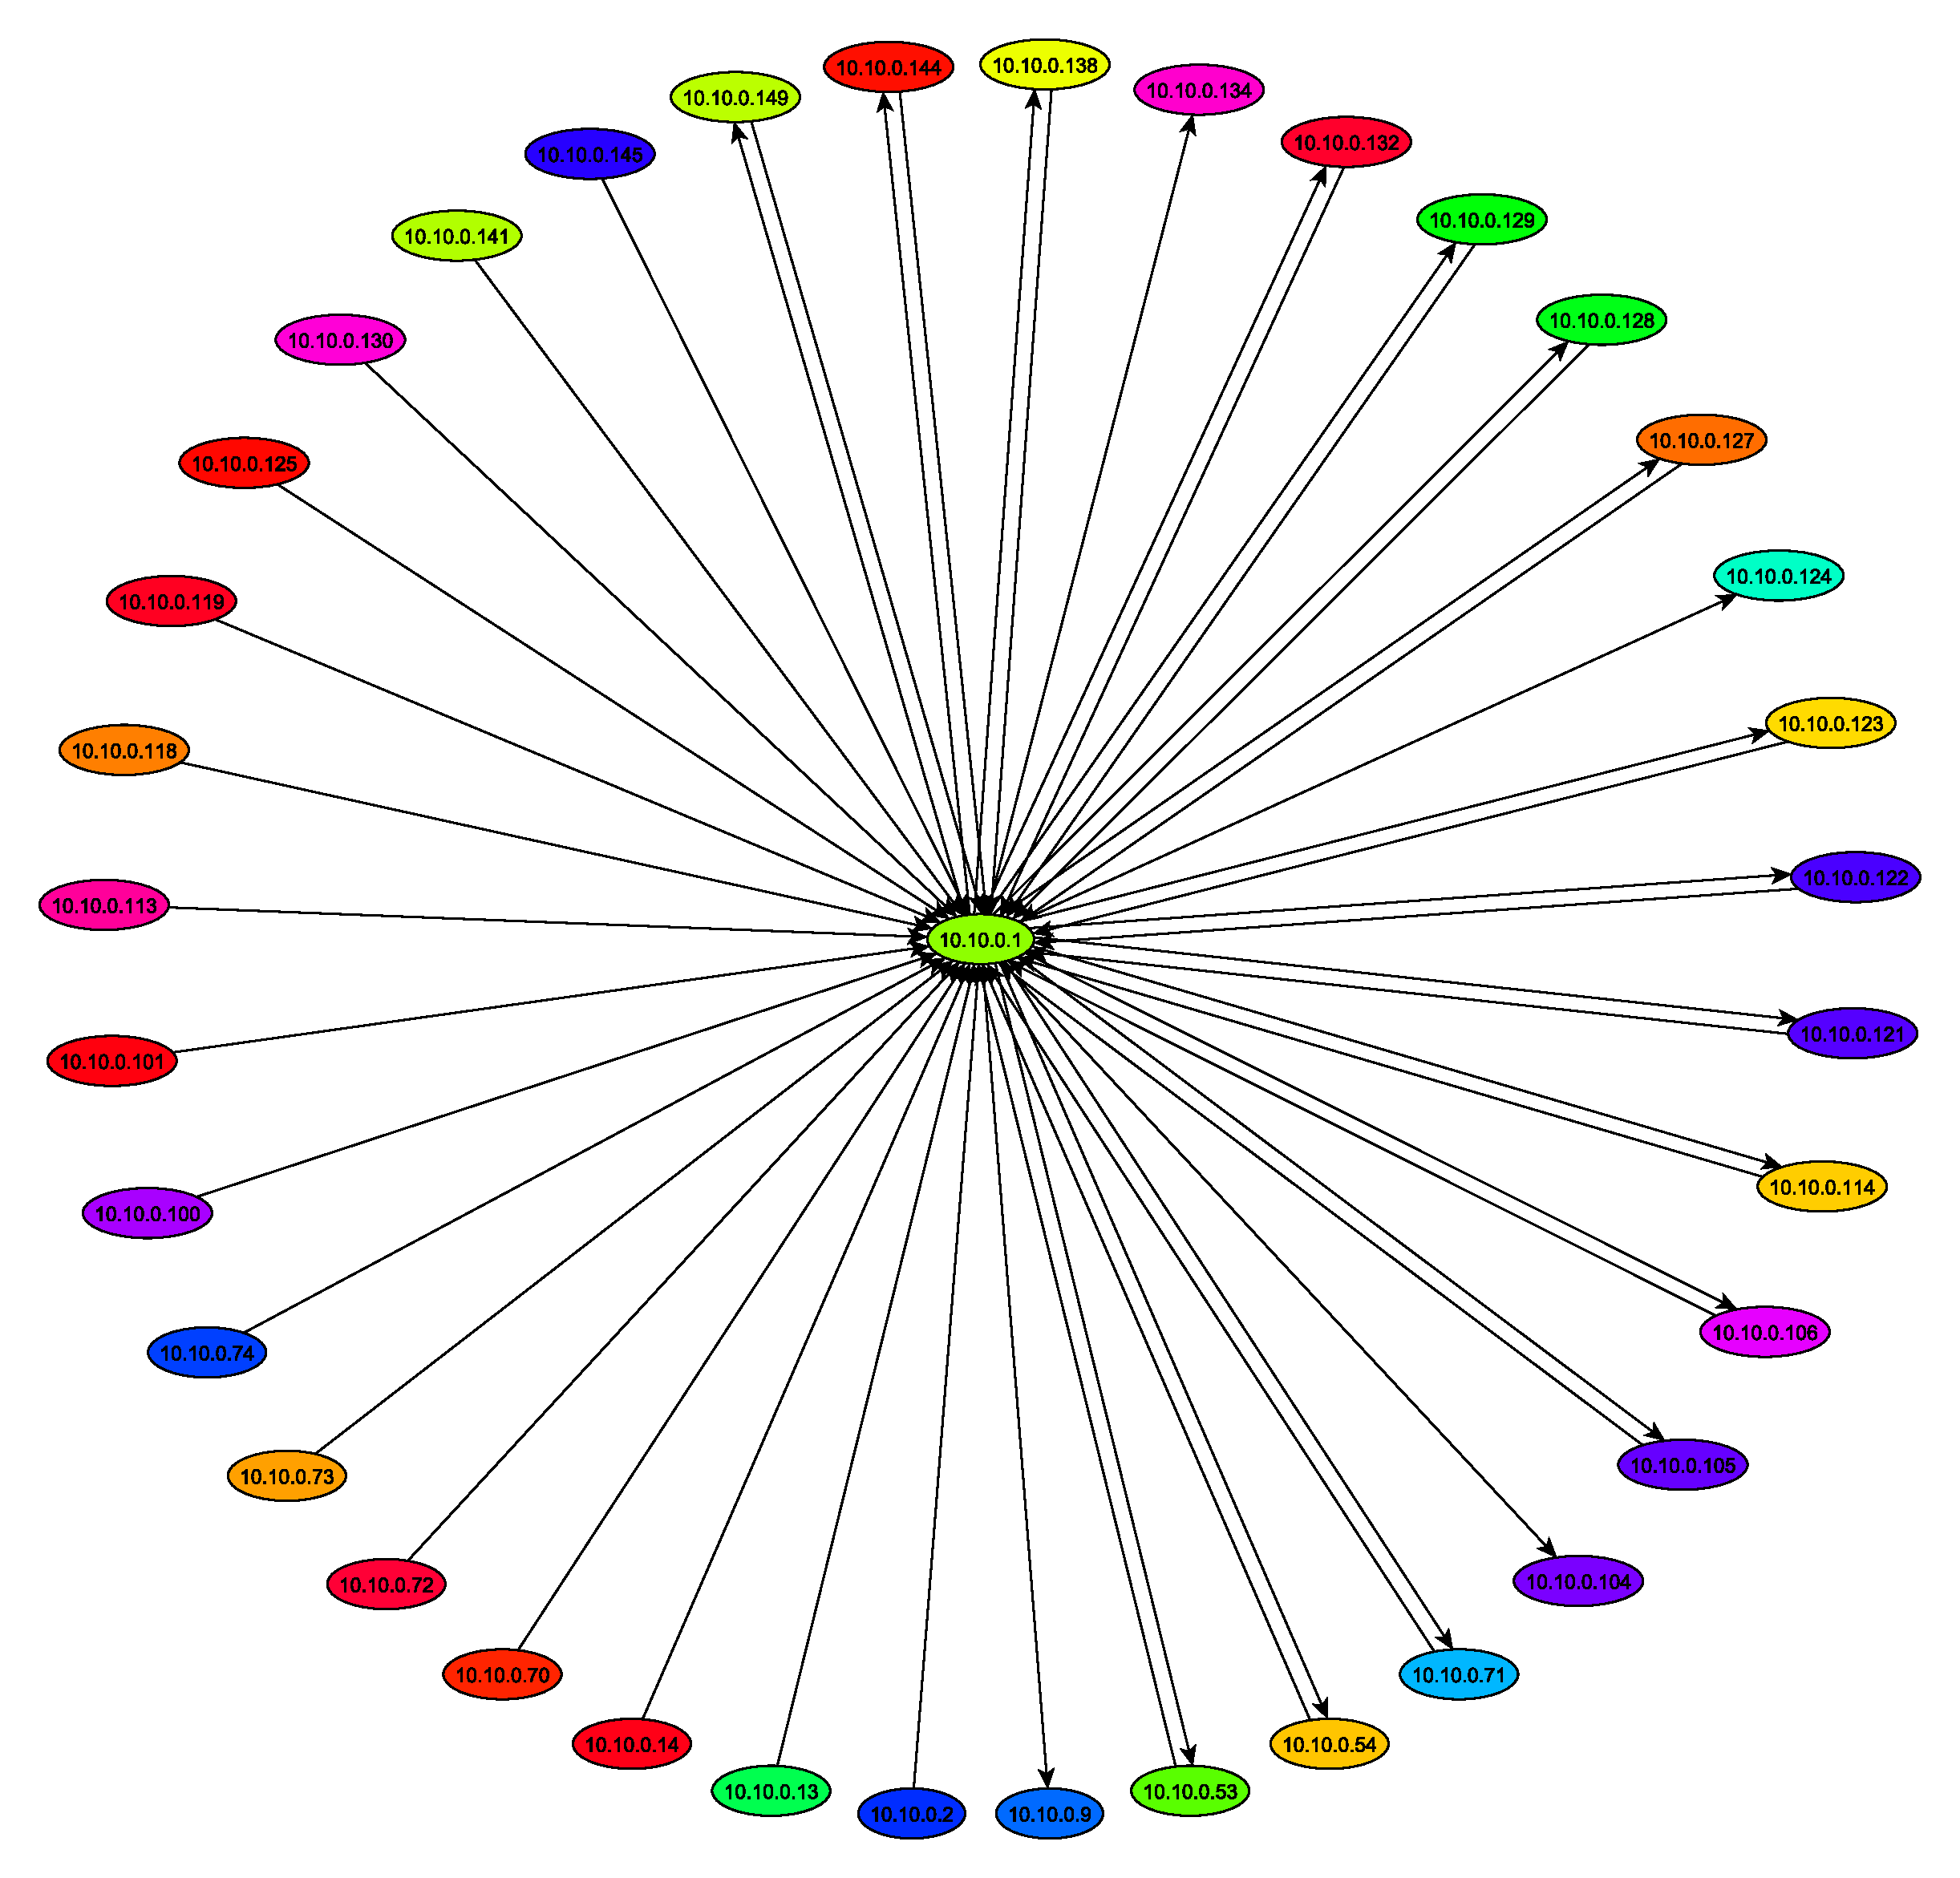
\includegraphics[width=0.5\textwidth]{img/graph/escenario_2/vecindad1.eps}
		\caption{Escenario 2 - Vecindad 10.10.0.1}
		\label{fig:escenario2_vecindad1}
	\end{figure}
    \begin{figure}[H]
		\centering
		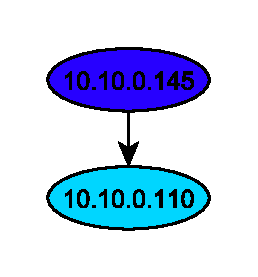
\includegraphics[width=0.35\textwidth]{img/graph/escenario_2/vecindad110.eps}
		\caption{Escenario 2 - Vecindad 10.10.0.110}
		\label{fig:escenario2_vecindad110}
	\end{figure}
    \begin{figure}[H]
		\centering
		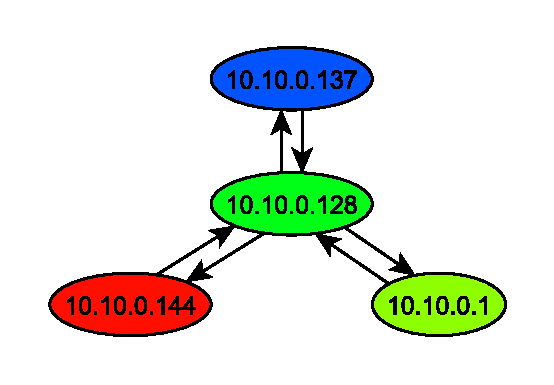
\includegraphics[width=0.5\textwidth]{img/graph/escenario_2/vecindad128.eps}
		\caption{Escenario 2 - Vecindad 10.10.0.128}
		\label{fig:escenario2_vecindad128}
	\end{figure}
    \begin{figure}[H]
		\centering
		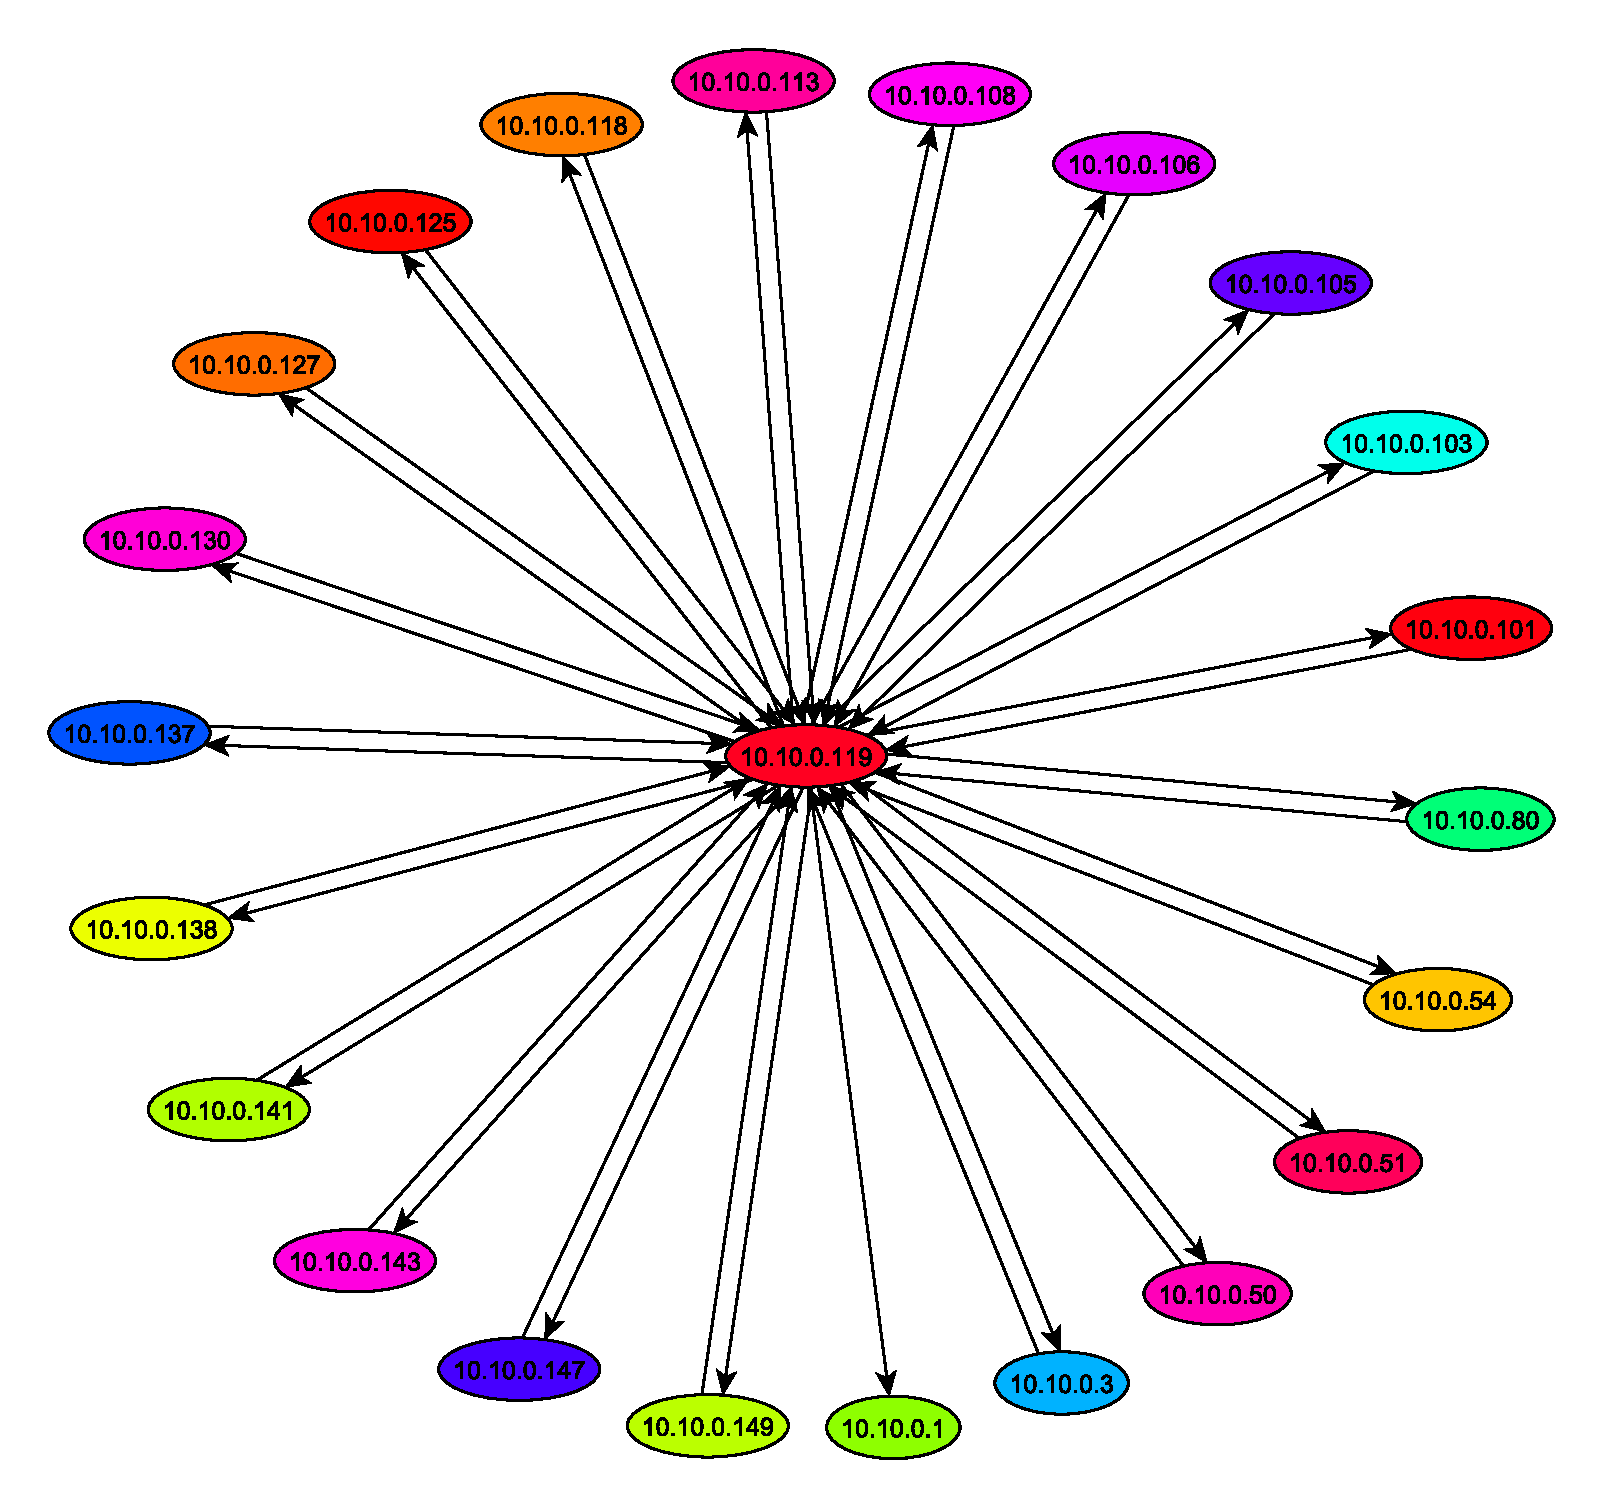
\includegraphics[width=0.5\textwidth]{img/graph/escenario_2/vecindad119.eps}
		\caption{Escenario 2 - Vecindad 10.10.0.119}
		\label{fig:escenario2_vecindad119}
	\end{figure}
    Acá notamos que 3 de las IPs tienen vecindades pobladas, lo que significa que seguramente sean nodos importantes en la red, mientras que en las otras dos se encuentran casí vacías.
    \par En el caso de la IP 10.10.0.110 vemos que esta no envió ningun pedido, por lo que es probable que no exista un host con esa IP, y que el equipo con IP 10.10.0.145 tuvierá configurado algún servicio que le pegue a la misma, y al no obtener respuesta, siguiera intentando continuamente, llenando de pedidos la red. Para corroborar una parte de esto, realizamos un ping hacia la IP 10.10.0.110 y vimos que efectivamente no existía.
    \par La IP 10.10.0.128 sabemos que existe en la red, ya que se ve que envía pedidos a otras IP, por lo que inspeccionamos con mayor detalle los pedidos dirigidas a esta. Nos llamo la atención que de los 714, 579 provenian del gateway. Aún más, los 579 se originaron en un rango 16 minutos, en los que la IP 10.10.0.128 no emitió ningún pedido. La conclusión que sacamos de esto es que probablemente esa dirección estuviera asignada a un teléfono celular, y que el dueño del mismo salió durante esos 15 minutos, por lo que el gateway comenzó a reintentar los pedidos al ver que no obtenía respuesta para esa IP.
        
	\subsubsection{Entrop\'ia}
		\par Entrop\'ia

\subsection{Conclusiones Preliminares}

\section{Escenario 3}
	\subsection{Descripci\'on del Escenario}
	\par En este escenario se monitorearon los paquetes ARP de la red Wi-Fi de acceso publico de un local de comida rápida en una zona muy concurrida de la ciudad de Buenos Aires.[Starbucks en Av. Callao]

	\par A la hora del analisis, mi posición es de completo desconocimiento sobre la naturaleza de la red, quienes intervienen en la misma y el accionar de los usuarios en ella.
    
	\par Se espera que en general las conexiones de los diversos dispositivos de la gente que concurre al local sea de algunos pocos minutos y busque simplemente acceder a internet, por lo cual se espera que la principal conmutación se de entre las IPs de estos dispositivos y el gateway.



\subsection{An\'alisis de datos obtenidos}
	\par La captura fue de 45 minutos y se enviaron 947 paquetes, el grafo dirigido de conexiones que se obtuvo fue el siguiente:

 %[-Grafo-]
 
 \begin{figure}[H]
		\centering
		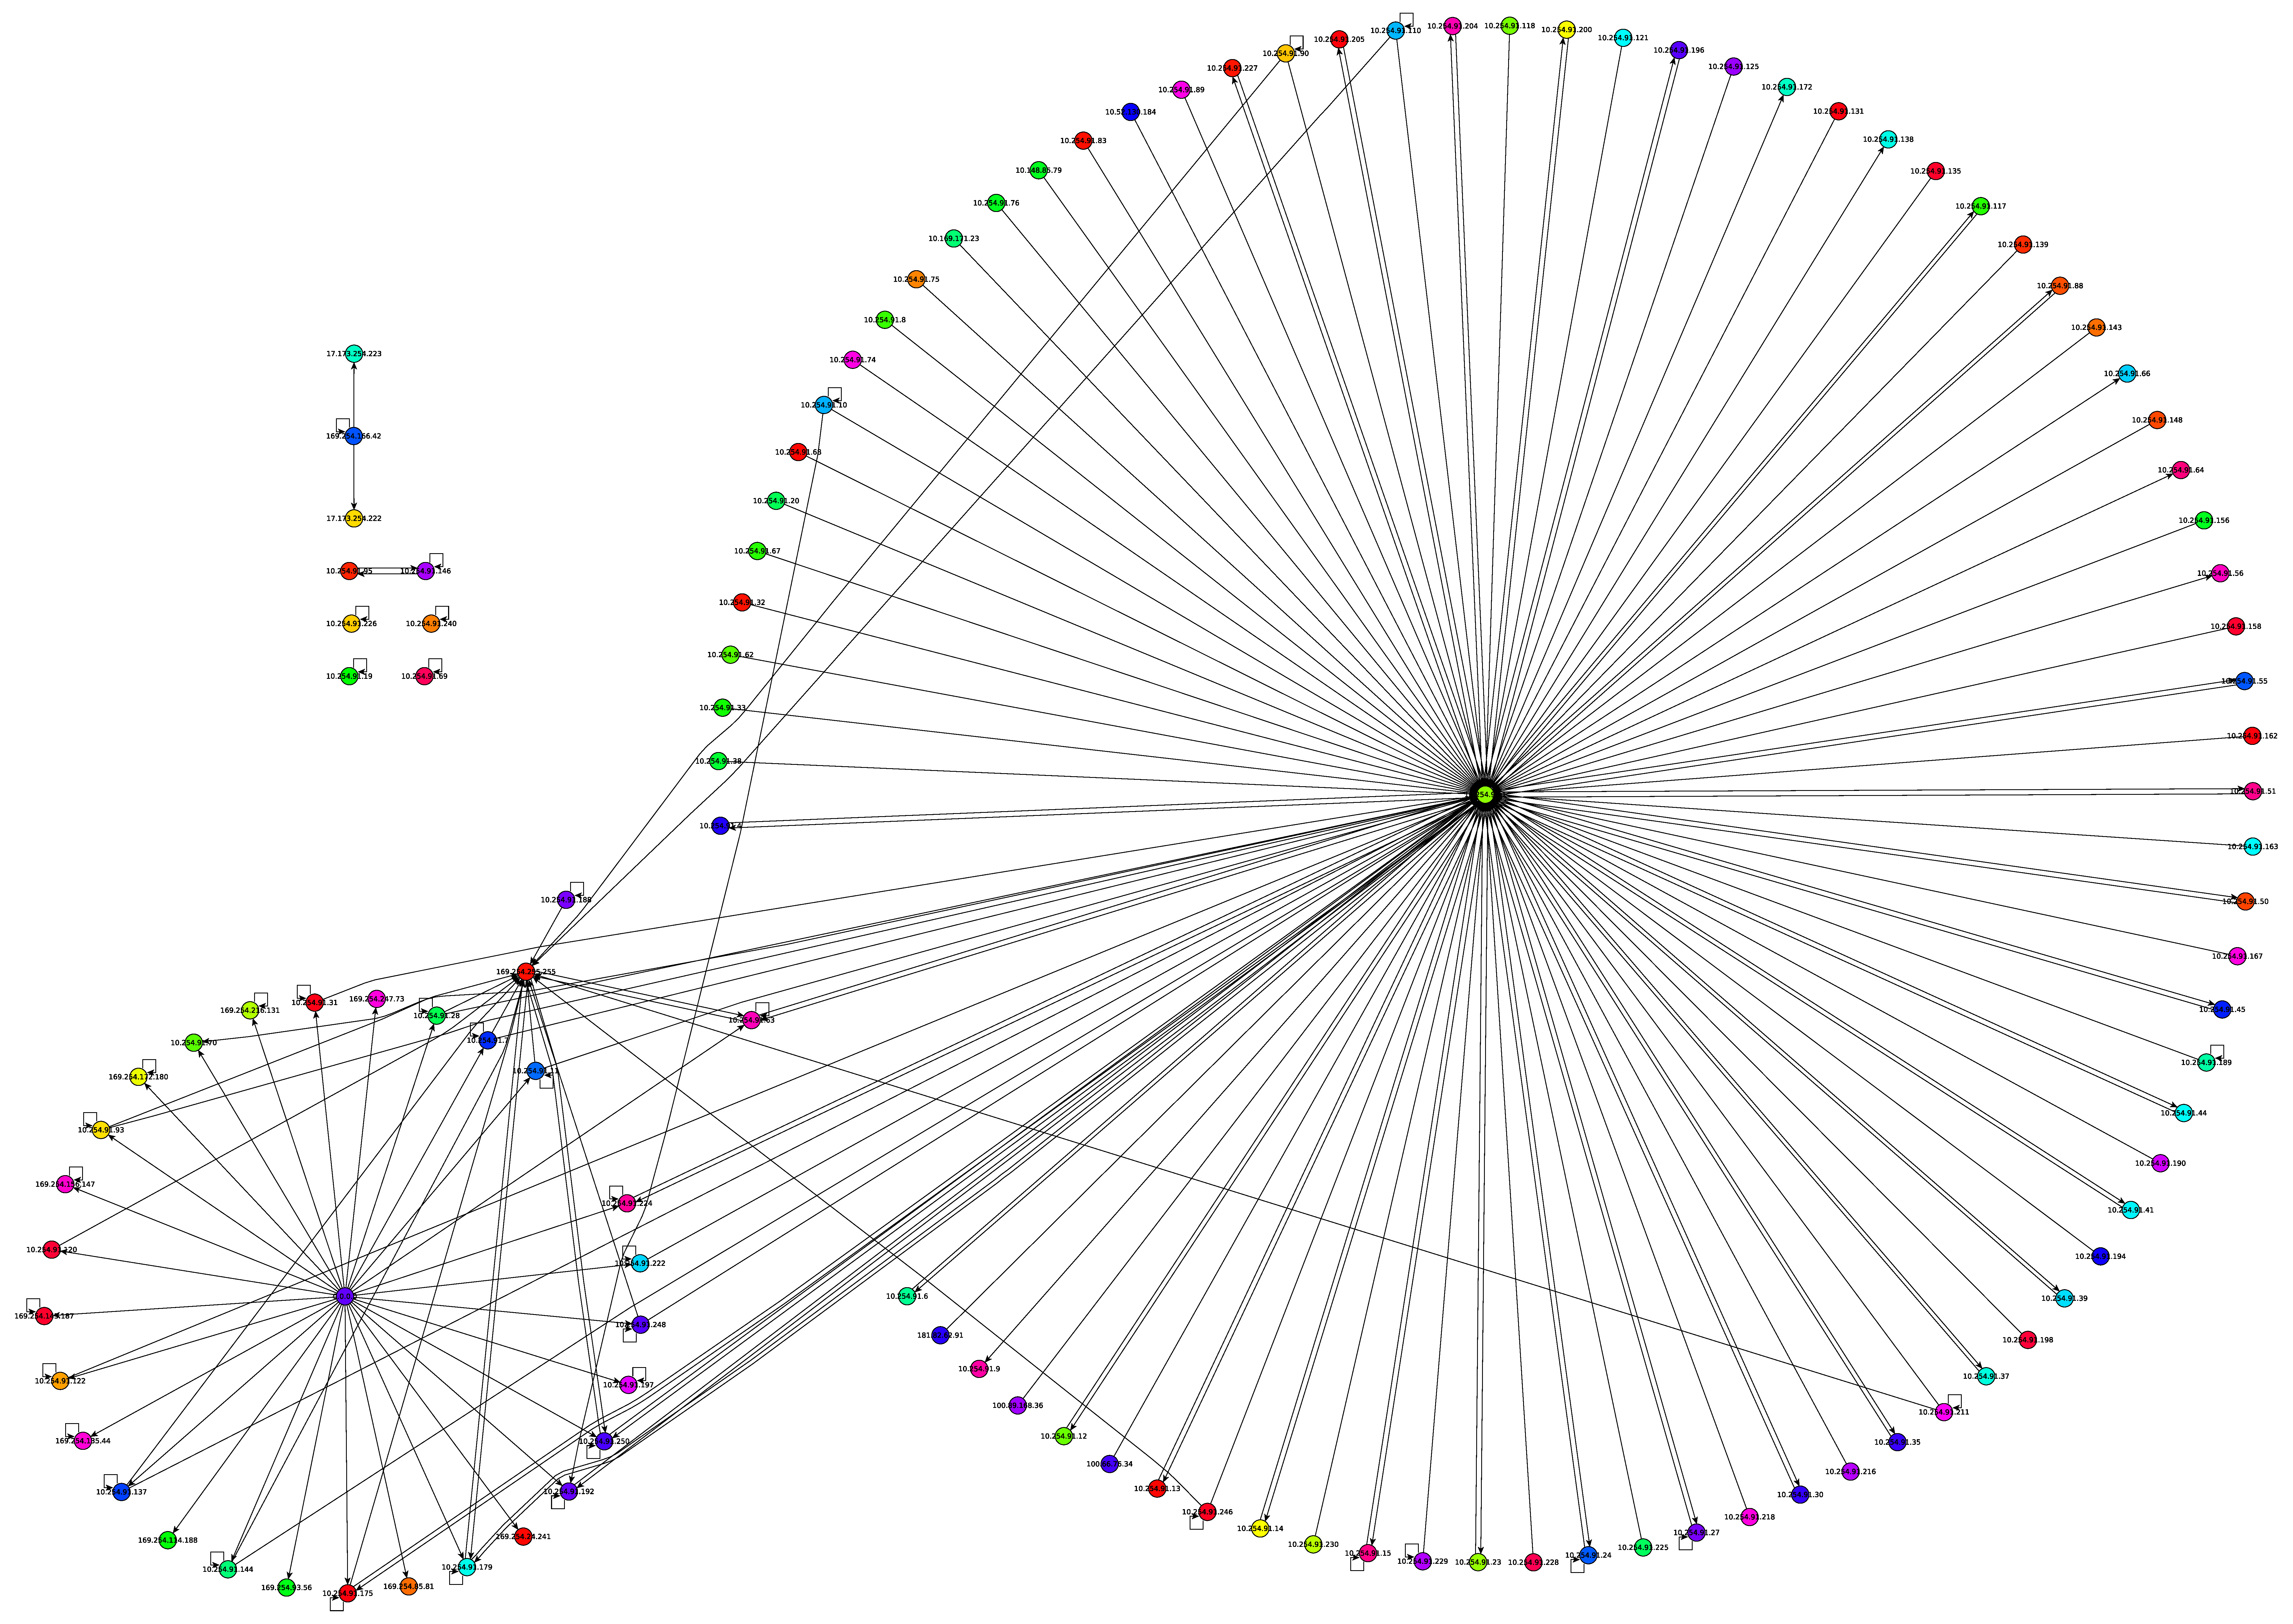
\includegraphics[width=0.5\textwidth]{img/graph/escenario_3/starbucks2.eps}
		\caption{Grafo de la red del Escenario 3}
		\label{fig:grafo_escenario3}
	\end{figure}

	\par Como el grafo es de gran tamaño vamos a considerar subgrafos donde se encuentran nodos interesantes para el analisis.

	\par Hay dos direcciones involucradas en gran parte del tráfico de paquetes, la 10.254.91.1 que  recibe y envia hacia una gran cantidad de IPs y la 169.254.255.255 que principalmente es destino.

	\par La primera se comporta como el gateaway, interactua con la mayoria de las IPs y es la más activa de la red.  

%[-Zoom a IP 10.254.91.1-]

\begin{figure}[H]
		\centering
		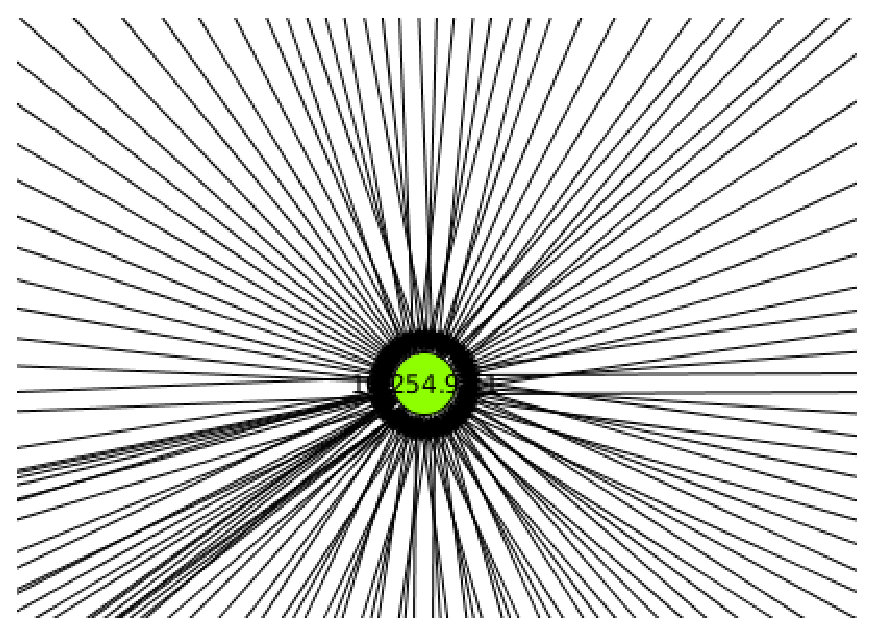
\includegraphics[width=0.5\textwidth]{img/graph/escenario_3/10254.eps}
		\caption{Ampliación en la cercan\'ia a 10.254.91.1}
		\label{fig:grafo_escenario3}
	\end{figure}


	\par La segunda es una direccion reservada  a la que los dispositivos envian paquetes ARP al no encontrar el servidor DHCP ya sea por recien conectarse o perder la ruta hacia el , el dispositivo se asigna una direccion para acceder y comunicarse a la red que usará hasta que se le asigne una IP mediante DHCP. 

%[-Vecindad de la IP 169.254.255.255-]

	\par Tambien se destaca que hay varias who-has con origen 0.0.0.0, esto se da porque al conectarse a la red ciertos dispositvo envian broadcast para ser detectados por el servidor y les asigne una IP, esto termina resultando en un paquete ARP con la IP asignada.

%[-Vecindad de la IP 0.0.0.0-]

	\par El resto de las direcciones se encuentran en el rango 10.254/16, lo cual es completamente razonable y 169.254/16 que es un caso más interesante, estas direcciones son conocidas como Link-local addresses, son direcciones reservadas asignadas en Windows cuando no puede establecer contacto con el servidor DHCP y se genera su propia IP mediante el direccionamiento conocido como APIPA.

	\par El sistema operativo intentará constantemente conectarse con DHCP y recibir una IP válida, mientras tanto los hosts con estas direcciones pueden comunicarse entre si dentro de la red, pero no con ninguno externo a la red local.

	\par Algunas otras caracteristicas del grafo son:

\begin{itemize}

\item Nodos Aislados:

	\par En el grafo se presentan nodos que podemos definir como aislados dado que no se conectan con el gateway 10.254.91.1.
Estos dispositivos se comunican entre sí, con si mismos, o con nadie como es el caso de 17.173.254.223 que no envia paquetes.

	\par  Como es minimamente necesario que envien un paquete a 10.254.91.1 apenas ingresan a la red, nos hace suponer que el host se encontraba conectado a la red antes de hacer el análisis y de esta forma obtuvieron su direccion.  

%[-Subgrafo con nodos aislados-]

\item Nodos Reflexivos:

	\par Podemos destacar nodos que envian paquetes a si mismos, algunos motivos por los que puede suceder esto es para actualizar la tabla ARP, para buscar duplicados de la direccion IP o cambios de la direccion MAC.Este envio de paquetes se conoce como Gratuitous ARP.

\end{itemize}
%http://wiki.wireshark.org/Gratuitous_ARP



	\subsubsection{Entrop\'ia}
		\par Entrop\'ia

\subsection{Conclusiones Preliminares}


\section{Escenario 4}
	\input{escenario4}

\section{Conclusiones}
	\IEEEPARstart{LL}{e}gados al final del trabajo expuesto, 


\printbibliography
\end{document}
